\documentclass[11pt,a4paper]{article}

\usepackage{fontspec}
\usepackage[french]{babel}
\usepackage[a4paper,margin=2.2cm,bottom=2.6cm]{geometry}
\usepackage{graphicx}
\usepackage{float}
\usepackage{booktabs}
\usepackage{tabularx}
\usepackage{array}
\usepackage[table]{xcolor}
\usepackage{caption}
\usepackage{enumitem}
\usepackage{titlesec}
\usepackage{fancyhdr}
\usepackage{hyperref}
\usepackage{xurl}

\setmainfont{texgyreheros}[
  Extension=.otf,
  UprightFont=*-regular,
  BoldFont=*-bold,
  ItalicFont=*-italic,
  BoldItalicFont=*-bolditalic]
\definecolor{accent}{HTML}{2A78D6}
\definecolor{ink2}{HTML}{52514E}
\hypersetup{colorlinks=true, linkcolor=accent, urlcolor=accent}
\graphicspath{{figures/}}

\titleformat{\section}{\Large\bfseries\color{accent}}{\thesection.}{0.6em}{}[\vspace{-0.4em}\color{accent}\rule{\linewidth}{0.8pt}]
\titleformat{\subsection}{\large\bfseries}{\thesubsection}{0.6em}{}
\titlespacing*{\section}{0pt}{1.6em}{0.9em}

\captionsetup{font={small,color=ink2}, labelfont=bf, justification=raggedright, singlelinecheck=false}
\setlist{itemsep=0.25em, topsep=0.4em}
\setlength{\parskip}{0.45em}
\renewcommand{\arraystretch}{1.25}
\newcolumntype{Y}{>{\raggedright\arraybackslash}X}

\pagestyle{fancy}
\fancyhf{}
\fancyhead[L]{\small\color{ink2} complaint-triage -- Rapport de cadrage}
\fancyhead[R]{\small\color{ink2} v0.0}
\fancyfoot[R]{\small\color{ink2}\thepage}
\renewcommand{\headrulewidth}{0.3pt}

\begin{document}

\hypersetup{pageanchor=false}
\begin{titlepage}
  \setlength{\parindent}{0pt}
  \vspace*{5cm}
  {\color{accent}\bfseries\large COMPLAINT-TRIAGE}\par\vspace{0.6cm}
  {\fontsize{30}{36}\selectfont\bfseries Rapport de cadrage}\par\vspace{0.5cm}
  {\Large\color{ink2} Priorisation des réclamations clients en banque de détail}\par
  \vfill
  {\color{accent}\rule{\linewidth}{1.2pt}}\par\vspace{0.3cm}
  {\color{ink2}
  Nathan Mang\\
  17 octobre 2026\\
  Version 0.0, avant tout développement}
  \vspace{2cm}
\end{titlepage}
\hypersetup{pageanchor=true}

\setcounter{tocdepth}{1}
\tableofcontents
\newpage

\section*{Synthèse}
\addcontentsline{toc}{section}{Synthèse}

Le service réclamations d'une banque de détail reçoit chaque mois des milliers de dossiers et les traite le plus souvent dans l'ordre d'arrivée. Pourtant, une minorité d'entre eux, environ un sur sept dans le périmètre étudié, se termine par une indemnisation financière du client. Ce sont les réclamations fondées. Quand elles attendent dans la file, le préjudice dure plus longtemps, le client peut saisir le médiateur ou le régulateur, et le délai de réponse réglementaire devient plus difficile à tenir.

Le projet complaint-triage propose un assistant de priorisation pour ce service. À l'arrivée d'une réclamation, il estime la probabilité qu'elle aboutisse à une indemnisation et la place dans la file en conséquence. Il propose ensuite une réponse appuyée sur des documents dont il cite la source, et il peut exécuter quelques actions encadrées, comme mettre à jour un statut ou alerter un responsable. S'il manque d'éléments pour agir, il refuse et explique pourquoi. L'outil change l'ordre de traitement. Il ne décide jamais de l'issue d'un dossier et n'en retire aucun de la file.

Le projet utilise uniquement des données publiques réelles : la base de réclamations du régulateur financier américain, le \emph{Consumer Financial Protection Bureau} (CFPB). Elle compte 18,5~millions de réclamations depuis 2011 et elle est mise à jour tous les jours. Je me limite à la banque de détail (cartes de crédit, comptes courants et comptes d'épargne), soit environ 16\,000 réclamations par mois en 2026.

Cette base a déjà servi à de nombreux projets publics, presque toujours sous la forme d'une étude ponctuelle dans un notebook. La situation a changé le 14 août 2026 : le CFPB a cessé de publier le texte des réclamations. Un modèle qui dépendait de ce texte ne peut plus être utilisé tel quel sur les nouvelles réclamations. Le projet part de cette contrainte. Il est conçu pour tourner en continu, sans le texte en production, et pour être évalué au fil de l'eau sur les décisions réelles des banques.

Le critère de succès est fixé avant toute modélisation. Je mesure la part des réclamations indemnisées qui se trouvent dans les 10~\% de la file traités en priorité, que j'appelle Capture@10~\%. Un tri aléatoire en capte 10~\%. Le modèle ne sera retenu que s'il fait nettement mieux qu'une règle métier simple, avec un seuil précisé en section~\ref{sec:criteres}. Dans le cas contraire, c'est la règle simple qui sera livrée, et l'échec du modèle sera documenté.

Le travail est découpé en six versions publiées sur GitHub, de la v0.1 à la v1.0, sur environ quatre mois. Chaque version s'accompagne d'une note de décision technique et d'un rapport comme celui-ci.

\section{Contexte}

\subsection{Le traitement des réclamations est encadré}

En France, l'Autorité de contrôle prudentiel et de résolution (ACPR) fixe les bonnes pratiques de traitement des réclamations dans la banque et l'assurance. Sa recommandation 2024-R-02 du 2 juillet 2024, qui remplace la 2022-R-01, demande de répondre « dans les meilleurs délais, et en tout état de cause dans un délai n'excédant pas deux mois ». Elle demande aussi d'exploiter les réclamations pour repérer et corriger les dysfonctionnements \cite{acpr2024,acpr2022}.

Aux États-Unis, le CFPB transmet les réclamations des consommateurs aux établissements concernés. Ceux-ci répondent en général sous 15~jours et peuvent donner une réponse définitive sous 60~jours \cite{cfpbprocess}. Le CFPB publie ensuite chaque réclamation, sans les informations qui identifient le consommateur, dans une base ouverte à tous.

Des deux côtés, une réclamation représente un coût potentiel (indemnisation, sanction, image) et une information utile sur ce qui ne fonctionne pas dans les produits et les processus.

\subsection{L'arrêt de la publication des récits}

Le 14 août 2026, le CFPB a annoncé qu'il ne publierait plus les récits des consommateurs, c'est-à-dire le texte libre où ils décrivent leur problème \cite{aba2026}. L'étude de faisabilité (section~\ref{sec:faisabilite}) en précise les effets :
\begin{itemize}
  \item l'API et l'export quotidien ne contiennent plus aucun récit, y compris pour les anciennes réclamations ;
  \item les données structurées (produit, motif, établissement, issue) sont toujours publiées chaque jour ;
  \item les récits publiés avant cette date restent disponibles dans une archive officielle, publiée au titre de la loi américaine sur l'accès aux documents administratifs \cite{foia}.
\end{itemize}

Pour un système de machine learning, la situation est concrète : une source de données utilisée par le modèle disparaît du jour au lendemain, et il faut continuer à fonctionner sans elle.

\subsection{Le client visé}

Le client est fictif, mais son besoin est réel : il s'agit du service réclamations d'une banque de détail. Le tableau~\ref{tab:parties} présente les personnes concernées par le projet.

\begin{table}[H]
\centering\small
\begin{tabularx}{\linewidth}{@{}l l Y@{}}
\toprule
Partie prenante & Rôle & Attente principale \\
\midrule
Responsable du service réclamations & Commanditaire & Traiter d'abord les dossiers importants et tenir les délais \\
Chargés de réclamations & Utilisateurs & Une file ordonnée et des réponses préparées, avec leurs sources \\
Conformité & Contrôle & Des décisions traçables, sans biais, et des délais respectés \\
Délégué à la protection des données & Contrôle RGPD & Ne traiter que les données nécessaires \\
Équipe data et informatique & Exploitation & Un système simple à maintenir, surveillé et peu coûteux \\
\bottomrule
\end{tabularx}
\caption{Parties prenantes}
\label{tab:parties}
\end{table}

\section{Problèmes et besoins}

\subsection{Problèmes constatés}

\begin{table}[H]
\centering\small
\begin{tabularx}{\linewidth}{@{}l Y Y@{}}
\toprule
& Problème & Conséquence \\
\midrule
P1 & Les réclamations sont traitées dans l'ordre d'arrivée & Un dossier fondé peut attendre derrière des dizaines de demandes simples \\
P2 & Le volume augmente : il a été multiplié par 2,7 entre janvier 2022 et septembre 2026 sur le périmètre (figure~\ref{fig:volume}) & À effectif constant, les délais s'allongent \\
P3 & Les réclamations fondées sont minoritaires, environ 14~\% & Elles sont difficiles à repérer à la lecture \\
P4 & Rédiger une réponse demande de retrouver la bonne procédure & Du temps perdu et des réponses hétérogènes \\
P5 & Les outils d'IA générative peuvent inventer une réponse & Un risque juridique qu'une banque ne peut pas accepter \\
P6 & Les sources de données changent sans préavis (arrêt des récits en 2026, nouvelle nomenclature en 2023) & Un modèle non surveillé se dégrade sans que personne ne s'en aperçoive \\
\bottomrule
\end{tabularx}
\caption{Problèmes constatés et leurs conséquences}
\end{table}

\subsection{Besoins}

\begin{enumerate}[label=B\arabic*.]
  \item Classer la file selon le risque qu'une réclamation soit fondée.
  \item Pouvoir justifier chaque priorité auprès de la conformité.
  \item Proposer une réponse qui cite ses sources, ou ne rien proposer.
  \item Automatiser les actions répétitives (mise à jour de statut, alerte), avec des garde-fous.
  \item Rester fiable dans le temps et signaler automatiquement les dérives.
\end{enumerate}

\subsection{Hors périmètre}

L'outil ne décide pas de l'issue d'une réclamation ni du montant d'une indemnisation. Il ne retire aucun dossier de la file : chaque réclamation reste traitée dans le délai réglementaire. Enfin, le projet n'utilise aucune donnée interne de banque, seulement les données publiques du CFPB.

\section{Enjeux}

\begin{table}[H]
\centering\small
\begin{tabularx}{\linewidth}{@{}l l Y@{}}
\toprule
Enjeu & Nature & Ce que l'outil doit garantir \\
\midrule
Réglementaire & Délais de réponse, traçabilité & Chaque décision et chaque action est enregistrée \\
Client & Corriger plus vite un préjudice réel & Les réclamations fondées remontent en tête de file \\
Financier & Limiter les recours au médiateur ou au régulateur & L'avance prise sur les dossiers fondés est mesurée \\
Éthique & Ne défavoriser aucun groupe de clients & Une analyse par sous-groupe est obligatoire avant la mise en service \\
Technique & Résister aux changements de données & Modèle de repli, surveillance et tests automatisés \\
\bottomrule
\end{tabularx}
\caption{Enjeux du projet}
\end{table}

Un point mérite d'être dit clairement. Un outil qui repère les réclamations susceptibles d'aboutir à une indemnisation pourrait aussi servir à freiner ces dossiers. L'outil est conçu dans l'autre sens, pour corriger plus vite le préjudice du client. La priorité ne sert qu'à avancer des dossiers, jamais à en retarder un au-delà du délai réglementaire. L'analyse par sous-groupe vérifie en plus que les clients que le CFPB signale comme vulnérables (étiquettes \emph{Older American} et \emph{Servicemember}) ne sont pas moins bien traités que les autres.

\section{Travaux existants}

Avant de concevoir la solution, j'ai recensé les projets publics qui utilisent la même base.

\begin{table}[H]
\centering\small
\begin{tabularx}{\linewidth}{@{}l Y Y@{}}
\toprule
Travail & Contenu & Limite pour notre besoin \\
\midrule
\emph{cfpb-monetary-relief} \cite{gh-kingston} & Prédiction de l'indemnisation à partir des récits (2023-2024) & Étude ponctuelle, pas de mise en production \\
\emph{consumer-finance-risk-analytics} \cite{gh-jskjames} & Régression logistique sur les données disponibles à la réception, application Streamlit & Pas de texte, pas de suivi dans le temps \\
\emph{cfpb-complaint-prediction} \cite{gh-ruhel} & XGBoost avec des variables extraites des récits par un LLM & Autre cible (escalade), pas de production \\
\emph{bank-complaint-classifier} \cite{hf-rakshith} & DistilBERT entraîné sur les récits & Un modèle seul, sans système autour \\
Travaux académiques \cite{arxiv2024} & Prédiction de l'indemnisation par forêts aléatoires et arbres de décision & Résultats modestes, approche hors ligne \\
\bottomrule
\end{tabularx}
\caption{Projets publics sur la base du CFPB}
\end{table}

La modélisation a donc déjà été explorée. Je la traite comme un point de départ à reproduire puis à dépasser, et non comme l'apport principal du projet. Aucun des travaux trouvés ne fait tourner un système en continu, ne gère l'arrêt des récits ou le délai d'arrivée des issues, ni ne propose un agent qui agit avec des garde-fous. Cette liste n'est sans doute pas complète et sera enrichie pendant le projet.

\section{Étude de faisabilité}
\label{sec:faisabilite}

\subsection{Méthode}

Les chiffres de cette section ont été produits le 17 octobre 2026 par un script versionné dans le dépôt, \nolinkurl{scripts/feasibility/collect_cfpb_feasibility_stats.py}. Il interroge l'API publique du CFPB, qui ne demande ni compte ni clé, et télécharge trois fichiers de l'archive officielle. Les données agrégées sont enregistrées dans \nolinkurl{docs/v0.0-cadrage/data/}, et n'importe qui peut relancer le calcul.

\subsection{Volume}

La base compte 18,5~millions de réclamations, tous produits confondus. Le \emph{credit reporting}, c'est-à-dire la contestation des rapports de crédit, en représente 84~\% en 2024 et 96~\% en octobre 2026. Ces réclamations visent les agences d'évaluation du crédit et non les banques de détail, je les exclus donc. Sur le périmètre retenu, le volume passe d'environ 6\,000 à environ 16\,000 réclamations par mois entre 2022 et 2026.

\begin{figure}[H]
\centering
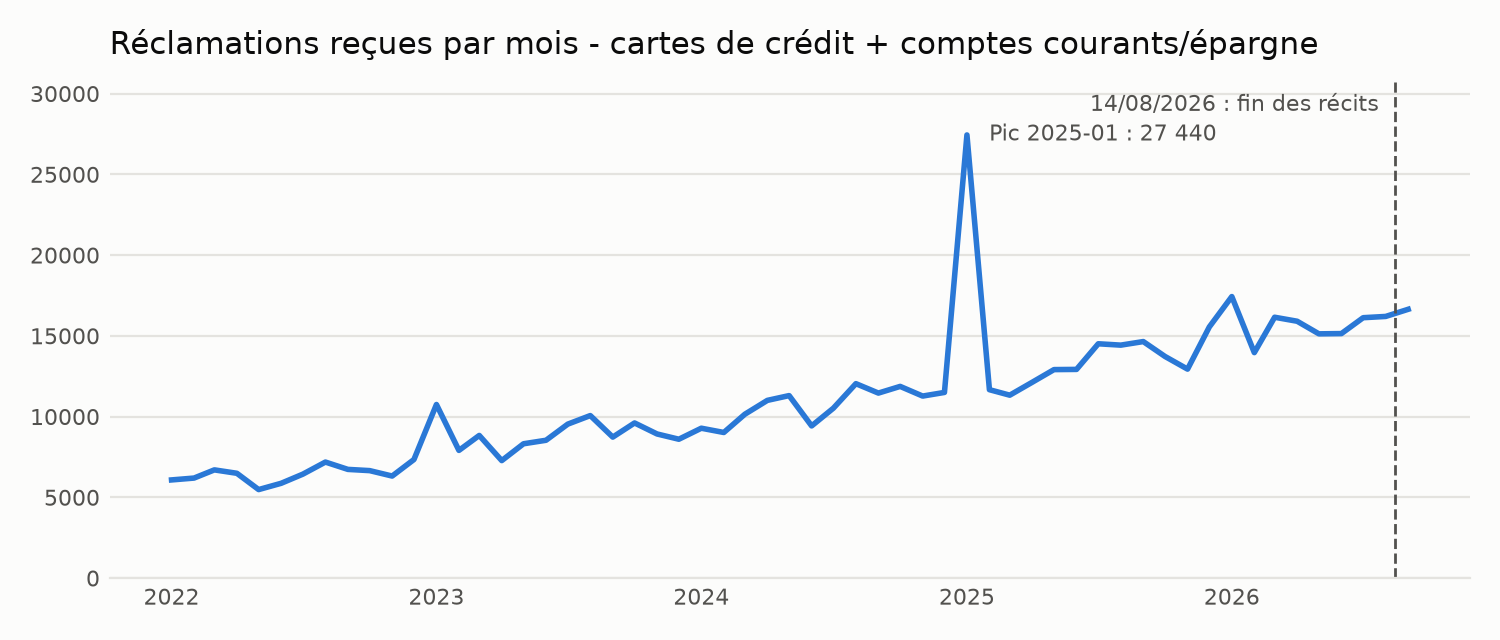
\includegraphics[width=\linewidth]{volume-mensuel-reclamations.png}
\caption{Réclamations reçues par mois sur le périmètre. Le pic de janvier 2025 (27\,440 réclamations, plus du double des mois voisins) reste à expliquer pendant l'exploration des données.}
\label{fig:volume}
\end{figure}

\subsection{Variable cible}

Chaque établissement indique l'issue de la réclamation dans la colonne \texttt{Company response to consumer}.

\begin{table}[H]
\centering\small
\begin{tabular}{@{}l r r r@{}}
\toprule
Produit (2025) & Réclamations & \shortstack[r]{Indemnisation\\financière} & \shortstack[r]{Correction\\non financière} \\
\midrule
Carte de crédit & 89\,978 & 12,7~\% & 20,6~\% \\
Compte courant ou d'épargne & 84\,195 & 10,6~\% & 4,8~\% \\
\addlinespace
\emph{Recouvrement de créances (comparaison)} & 283\,203 & 0,2~\% & 25,6~\% \\
\emph{Crédit immobilier (comparaison)} & 24\,697 & 1,7~\% & 2,7~\% \\
\bottomrule
\end{tabular}
\caption{Issue des réclamations par produit en 2025}
\end{table}

Sur le périmètre, 14,0~\% des réclamations reçues entre janvier 2022 et juin 2026 ont abouti à une indemnisation financière. La cible est rare, sans l'être au point de rendre le problème insoluble, ce qui correspond bien à une tâche de priorisation.

\begin{figure}[H]
\centering
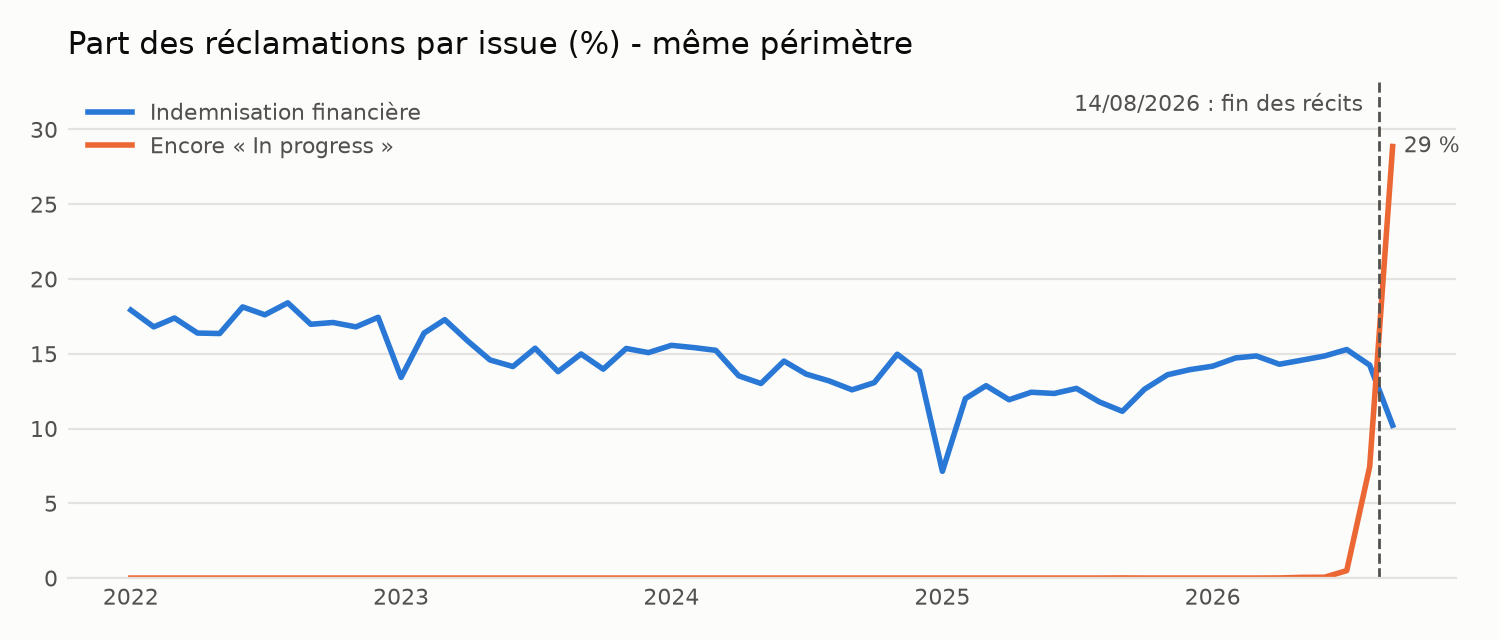
\includegraphics[width=\linewidth]{issues-des-reclamations-par-mois.png}
\caption{Part des réclamations indemnisées et des dossiers encore en cours, par mois de réception.}
\label{fig:issues}
\end{figure}

La figure~\ref{fig:issues} conduit à deux décisions. D'abord, le taux d'indemnisation varie dans le temps : il passe d'environ 18~\% début 2022 à 12-15~\% ensuite. Un modèle entraîné sur 2022 serait mal calibré en 2026. Il faut donc découper les données strictement dans le temps et surveiller le modèle une fois en service.

Ensuite, l'issue d'une réclamation n'est connue qu'après la réponse de la banque. Fin septembre, 29~\% des réclamations reçues dans le mois sont encore « In progress ». Ce chiffre tombe à 7,4~\% après deux mois et à 0,5~\% après trois. La baisse apparente du taux d'indemnisation sur les derniers mois vient de là, et non d'un vrai changement. J'en tire une règle : une réclamation n'entre dans l'entraînement que 90~jours après sa réception. Ce délai sera ajusté pendant l'exploration.

\subsection{Le texte des réclamations}

\begin{table}[H]
\centering\small
\begin{tabular}{@{}l r r r@{}}
\toprule
Période (archive officielle) & Réclamations du périmètre & Avec récit & Longueur médiane \\
\midrule
Mars-avril 2025 & 23\,451 & 51~\% & 162 mots \\
Juillet 2026 & 15\,990 & 24~\% & 209 mots \\
Août 2026 & 15\,548 & 0~\% & -- \\
\bottomrule
\end{tabular}
\caption{Présence du récit client dans l'archive}
\end{table}

\begin{figure}[H]
\centering
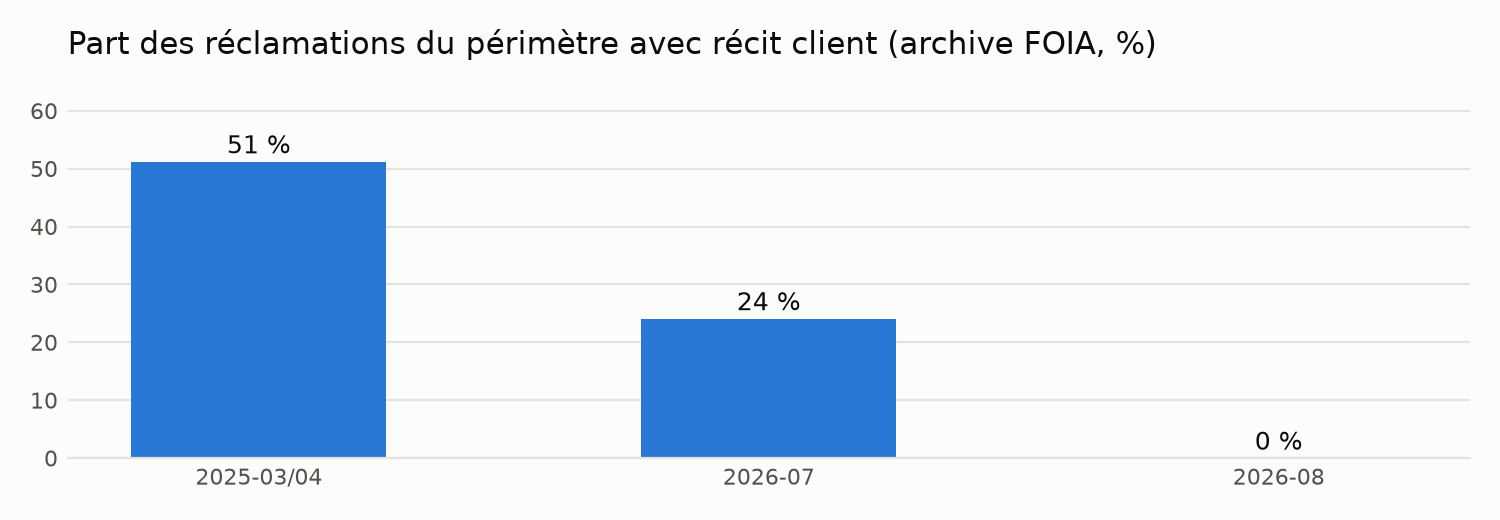
\includegraphics[width=\linewidth]{couverture-des-recits-clients.png}
\caption{Part des réclamations avec récit. Un récit n'est publié qu'après la réponse de la banque, donc les derniers mois avant l'arrêt n'ont jamais été complétés.}
\end{figure}

En 2025, environ 6\,000 récits par mois sont utilisables (mesure faite sur mars et avril), soit plusieurs dizaines de milliers par an sur le périmètre. C'est assez pour entraîner un modèle de langage. Le volume exact sur tout l'historique sera mesuré en v0.1. En revanche, aucune nouvelle réclamation n'aura de texte, et le modèle de production devra s'en passer.

\subsection{Pièges repérés}

\begin{table}[H]
\centering\small
\begin{tabularx}{\linewidth}{@{}l Y Y@{}}
\toprule
Piège & Description & Parade \\
\midrule
Fuite d'information & Certaines colonnes ne sont connues qu'après coup : réponse publique de la banque, respect du délai, date de transmission & Liste fermée des variables disponibles à la réception, vérifiée par un test automatique \\
Changement de nomenclature & En 2023, « Credit card or prepaid card » a été séparé en « Credit card » et « Prepaid card » & Table de correspondance versionnée et testée \\
Anomalie de janvier 2025 & Volume doublé et taux d'indemnisation divisé par deux & Analyse pendant l'exploration, puis exclusion ou pondération documentée \\
Issues pas encore connues & Les dossiers récents n'ont pas encore d'issue & Règle des 90~jours \\
Effet de l'établissement & Le taux d'indemnisation varie beaucoup d'une banque à l'autre & Traitement prudent de la variable, évaluation par établissement \\
\bottomrule
\end{tabularx}
\caption{Pièges identifiés dans les données}
\end{table}

\subsection{Conclusion}

Le projet est faisable. Les données sont réelles, publiques, volumineuses et datées, la cible est exploitable et de nouvelles réclamations arrivent chaque jour. La dérive, le délai des issues et la disparition du texte compliquent le travail, mais ce sont justement les problèmes que le projet veut traiter.

\section{Solution proposée}

\subsection{Architecture}

\begin{figure}[H]
\centering
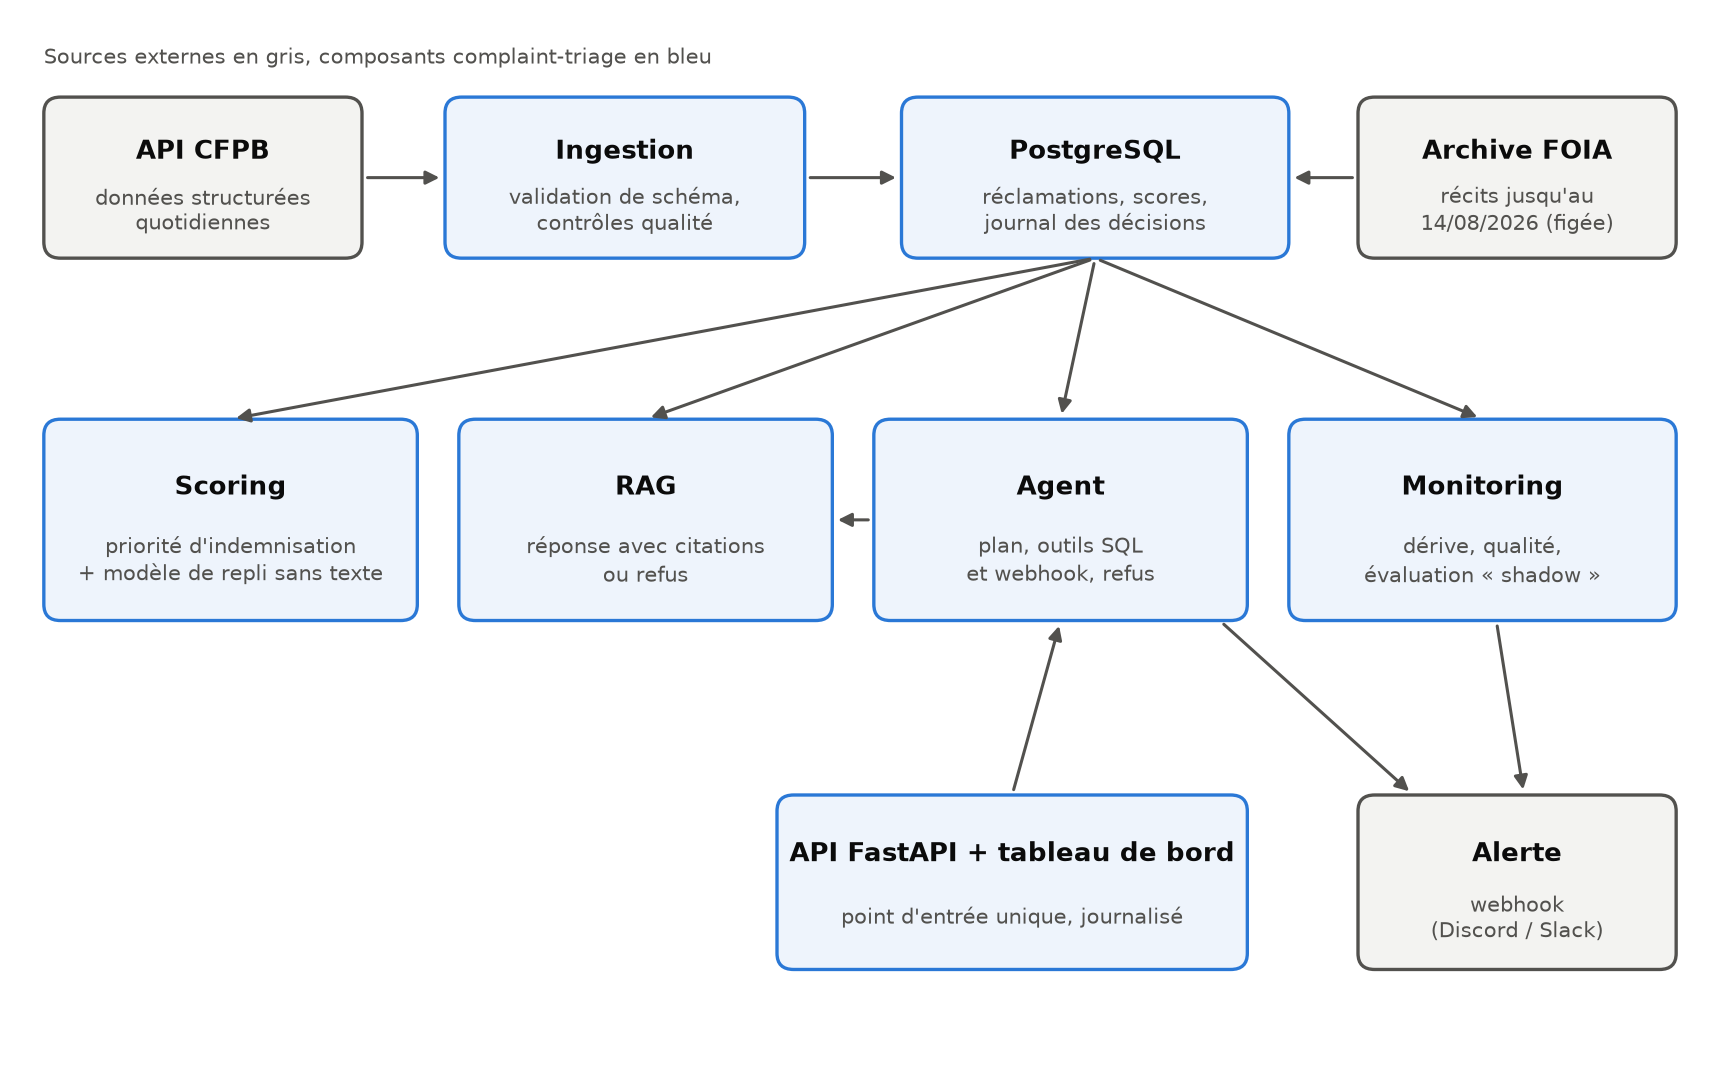
\includegraphics[width=0.95\linewidth]{architecture-cible.png}
\caption{Architecture cible. Les deux sources officielles alimentent une base PostgreSQL. L'API fait appel à l'agent, qui s'appuie sur le scoring et le RAG. L'agent et le monitoring peuvent envoyer des alertes.}
\end{figure}

\subsection{Les composants}

\begin{table}[H]
\centering\small
\begin{tabularx}{\linewidth}{@{}l Y l@{}}
\toprule
Composant & Rôle & Besoins \\
\midrule
Scoring & Estime la probabilité d'indemnisation à la réception. Un modèle XGBoost sur les données structurées sert en production. Un modèle de langage entraîné sur l'archive mesure ce que le texte apporte. & B1, B2 \\
RAG & Recherche dans une base documentaire (procédures internes simulées, textes réglementaires publics) les passages utiles, puis propose une réponse qui les cite, ou refuse & B3 \\
Agent & Lit une réclamation, interroge la base avec des requêtes SQL paramétrées (en lecture seule par défaut), met à jour un statut, envoie une alerte. Il annonce son plan et refuse en cas d'ambiguïté. & B4 \\
Monitoring & Contrôle la qualité des données entrantes et la dérive, compare chaque prédiction à l'issue réelle quand elle arrive, et alerte & B5 \\
\bottomrule
\end{tabularx}
\caption{Rôle de chaque composant}
\end{table}

\subsection{Évaluation en mode « shadow »}

Le projet n'a pas de vrais utilisateurs. Pour mesurer sa performance en conditions réelles, il fonctionne en mode « shadow » : chaque jour, il attribue un score aux nouvelles réclamations comme s'il était en service. Quelques semaines plus tard, une fois les réponses des banques publiées, il compare ses prédictions aux issues réelles. On obtient ainsi une mesure continue et honnête, sans que personne n'utilise l'outil.

\section{Critères de succès}
\label{sec:criteres}

Les seuils ci-dessous sont fixés avant toute modélisation, pour éviter de les ajuster ensuite en fonction des résultats.

\subsection{Indicateur principal}

L'indicateur principal est la Capture@10~\% : sur une semaine de réclamations, la part des dossiers finalement indemnisés qui figurent dans les 10~\% les mieux classés. Elle répond directement à la question du responsable : si mon équipe traite d'abord un dossier sur dix, combien de dossiers fondés passent en premier ?

Un tri aléatoire donne 10~\%. Ce n'est pas la bonne référence, car n'importe quelle règle de bon sens fait mieux. Je compare donc le modèle à une règle métier, appelée H0 : classer les réclamations selon le taux d'indemnisation historique de leur combinaison produit, motif et sous-motif, calculé sur la période d'entraînement. C'est ce que ferait un responsable expérimenté avec un tableur.

\subsection{Seuils par version}

Si le seuil de la v0.1 n'est pas atteint, la règle H0 devient le moteur de priorisation et le reste du système (RAG, agent, production) est construit autour d'elle. Le résultat négatif est alors documenté comme n'importe quel autre résultat.

\begin{table}[H]
\centering\small
\begin{tabularx}{\linewidth}{@{}l Y Y@{}}
\toprule
Version & Critère & Seuil \\
\midrule
v0.1 & Capture@10~\% du modèle structuré, sur la période de test la plus récente dont les issues sont connues & Au moins H0 + 5 points, et borne basse de l'intervalle de confiance à 95~\% (bootstrap) au-dessus de H0 \\
v0.1 & Apport du texte, sur la période où il existe & Gardé si le PR-AUC gagne au moins 0,02, sinon résultat négatif documenté \\
v0.1 & Équité : rapport des Capture@10~\% entre sous-groupes (\emph{Older American}, \emph{Servicemember}, produit) & Entre 0,8 et 1,25 \\
v0.1 & Calibration & Erreur de calibration (ECE) inférieure à 0,05 \\
v0.2 & Réponses du RAG qui citent au moins une source vérifiable & 100~\% \\
v0.2 & Refus sur des questions hors du corpus (jeu de test dédié) & Au moins 95~\% \\
v0.4 & Bon outil choisi par l'agent sur 20 à 25 scénarios écrits à l'avance & Au moins 90~\% \\
v0.4 & Refus attendus effectivement refusés & 100~\% \\
v1.0 & Temps de réponse du scoring (95\textsuperscript{e} centile) & Moins de 500~ms \\
v1.0 & Coût mensuel d'exploitation & Moins de 20~€ (budget visé) \\
\bottomrule
\end{tabularx}
\caption{Seuils de décision fixés avant la modélisation}
\end{table}

\clearpage
\section{Choix techniques}

\begin{table}[H]
\centering\small
\begin{tabularx}{\linewidth}{@{}l Y Y Y@{}}
\toprule
Besoin & Choix & Raison & Alternative écartée \\
\midrule
Langage & Python 3.12, mypy strict & Standard du domaine, le typage détecte des erreurs avant l'exécution & -- \\
Environnement & uv, pyproject.toml & Installation rapide et reproductible & pip et requirements.txt, moins stricts sur les versions \\
Qualité & ruff, pre-commit, pytest & Les contrôles bloquent les erreurs avant le commit, puis en CI & flake8 et black, deux outils pour le même travail \\
Modèles & scikit-learn, XGBoost, Transformers & Référence solide sur données tabulaires et sur le texte & Réseau de neurones tabulaire, rarement meilleur et moins explicable \\
Suivi des essais & MLflow & Garde la trace de chaque expérience & Un tableur, non reproductible \\
Base de données & PostgreSQL & Courant en entreprise, requêtes paramétrées & SQLite, peu représentatif d'un environnement de production \\
Recherche vectorielle & pgvector ou FAISS (choix en v0.2) & pgvector évite une base de plus, FAISS est déjà maîtrisé & Base vectorielle dédiée, un service de plus à exploiter \\
Agent & LangGraph & Les étapes (plan, outils, refus) sont explicites dans un graphe & Une boucle écrite à la main, plus difficile à relire \\
API & FastAPI & Validation des entrées par schémas, documentation générée & Flask, validation à écrire soi-même \\
Industrialisation & Docker, GitHub Actions & Lint, tests, build et déploiement, bloquants en cas d'échec & -- \\
Hébergement & GCP Cloud Run & Facturation à l'usage, arrêt automatique sans trafic & Machine virtuelle permanente, coût fixe \\
Rapports & LaTeX, compilé avec Tectonic & Rapports reproductibles par script, aussi en CI & Traitement de texte, non versionnable \\
\bottomrule
\end{tabularx}
\caption{Choix techniques et alternatives}
\end{table}

Quelques règles s'appliquent à tout le code. Aucun secret n'est écrit dans le code : les clés passent par des variables d'environnement, le fichier \texttt{.env} n'est jamais commité et un \texttt{.env.example} documente les variables attendues. Les requêtes SQL sont toujours paramétrées. Toute entrée est validée avant d'être transmise à un outil, et la logique métier reste séparée des routes de l'API.

\section{Démarche et planning}

\begin{table}[H]
\centering\small
\begin{tabularx}{\linewidth}{@{}l Y l@{}}
\toprule
Version & Contenu & Durée estimée \\
\midrule
v0.0 Cadrage & Ce rapport et l'étude de faisabilité & 1 semaine \\
v0.1 Données et scoring & Collecte automatisée, contrôles de qualité, exploration, règle H0, XGBoost, modèle de langage, analyse par sous-groupe & 3 à 4 semaines \\
v0.2 RAG & Corpus documentaire, recherche vectorielle, réponses avec citations ou refus & 2 semaines \\
v0.3 Agent & Boucle de planification, outils SQL et webhook, gestion des erreurs, refus argumentés & 3 semaines \\
v0.4 Qualité & Tests unitaires par outil, 20 à 25 scénarios d'évaluation intégrés à la CI & 2 semaines \\
v0.5 Industrialisation & Dockerfile, chaîne CI/CD complète & 1 à 2 semaines \\
v1.0 Production & Déploiement sur Cloud Run, collecte quotidienne, mode shadow, tableau de bord & 2 semaines \\
v1.1 et suivantes & Une amélioration toutes les une à deux semaines & En continu \\
\bottomrule
\end{tabularx}
\caption{Planning prévisionnel}
\end{table}

La durée totale jusqu'à la v1.0 est estimée à environ quatre mois. Chaque version donne lieu à une release GitHub avec son tag, une mise à jour du CHANGELOG, une note de décision technique dans \texttt{docs/adr/} et un rapport PDF. Les commits sont courts et leurs messages expliquent la raison du changement. Chaque fonctionnalité est développée sur sa propre branche et relue avant d'être fusionnée. À partir de la v0.1, la CI bloque toute fusion si le lint ou les tests échouent. Avant chaque version, j'écris la liste des essais prévus, leur ordre et le critère qui permet d'arrêter.

\section{Business case}

Ce business case est un exercice de cadrage pour une banque fictive. Les données du projet sont américaines, et chaque paramètre ci-dessous est une hypothèse à remplacer par les chiffres réels d'un établissement.

\begin{table}[H]
\centering\small
\begin{tabularx}{\linewidth}{@{}l l Y@{}}
\toprule
Paramètre & Hypothèse & Origine \\
\midrule
Réclamations reçues par mois & 2\,000 & Ordre de grandeur supposé pour une banque régionale \\
Part de réclamations fondées & 14~\% & Taux observé sur le périmètre (section~\ref{sec:faisabilite}) \\
Capacité de traitement prioritaire & 10~\% des dossiers & Paramètre de fonctionnement du service \\
Capture@10~\% atteinte & 30~\% & Hypothèse à vérifier en v0.1 (le hasard donne 10~\%) \\
\bottomrule
\end{tabularx}
\caption{Hypothèses du business case}
\end{table}

Avec ces hypothèses, la banque reçoit 280 réclamations fondées par mois. Dans l'ordre d'arrivée, 28 d'entre elles se retrouvent dans la file prioritaire. Avec une Capture@10~\% de 30~\%, elles seraient 84, soit 56 dossiers fondés de plus traités en premier chaque mois.

La valeur financière se calcule en multipliant ce nombre de dossiers par le coût évité pour chaque dossier traité tôt : recours au médiateur, préjudice qui se prolonge, risque de dépasser le délai. Ce coût dépend de chaque établissement et doit être estimé avec lui. Je ne le chiffre pas ici, faute de source fiable.

Côté dépenses, l'hébergement et les appels à un modèle de langage sont plafonnés à environ 20~€ par mois. L'essentiel du temps passé se concentre sur les quatre mois de construction, suivis d'une maintenance légère.

\section{Risques}

\begin{table}[H]
\centering\small
\begin{tabularx}{\linewidth}{@{}Y l l Y@{}}
\toprule
Risque & Probabilité & Impact & Mesure prévue \\
\midrule
Le modèle ne bat pas la règle H0 & Moyenne & Moyen & Seuil fixé à l'avance, H0 livrée et résultat documenté \\
Fuite d'information dans les variables & Élevée sans contrôle & Élevé & Liste fermée de variables, testée automatiquement \\
Nouveau changement des données du CFPB & Moyenne & Élevé & Contrôles de schéma à la collecte, alertes, modèle de repli \\
Biais envers un groupe de clients & Moyenne & Élevé & Analyse par sous-groupe bloquante (section~\ref{sec:criteres}) \\
L'agent exécute une action non voulue & Faible & Élevé & Lecture seule par défaut, validation des entrées, refus testés à 100~\% \\
Le modèle de langage invente une réponse & Moyenne & Élevé & Citation obligatoire, refus en cas de doute, évaluation automatique \\
Dépassement du budget cloud & Faible & Faible & Arrêt automatique sans trafic, plafonds de facturation \\
Données personnelles dans les récits & Faible (anonymisés par le CFPB) & Moyen & Aucun récit brut dans le dépôt, uniquement des agrégats, aucune tentative de réidentification \\
\bottomrule
\end{tabularx}
\caption{Principaux risques}
\end{table}

Sur le plan réglementaire, un outil d'aide à la priorisation des réclamations ne figure pas, à ma lecture, parmi les usages à haut risque listés par le règlement européen sur l'IA, contrairement à l'évaluation de la solvabilité. Le projet en reprend tout de même les bonnes pratiques : traçabilité, supervision humaine et documentation. Dans un contexte réel, ce point devrait être confirmé par un juriste.

\section{Prochaines étapes}

\begin{enumerate}
  \item Valider ce cadrage : périmètre, indicateurs et seuils.
  \item Initialiser le dépôt : structure, outils de qualité, premier commit et tag \texttt{v0.0}.
  \item Démarrer la v0.1 par la collecte automatisée et le contrôle des données, puis explorer les points relevés dans les pièges identifiés.
\end{enumerate}

\appendix
\newpage

\section{Variables disponibles à la réception}

\begin{table}[H]
\centering\small
\begin{tabularx}{\linewidth}{@{}l l Y@{}}
\toprule
Variable & Connue à la réception & Remarque \\
\midrule
Date received & Oui & Sert au découpage temporel, pas comme variable du modèle \\
Product, Sub-product & Oui & Nomenclature à harmoniser (2023) \\
Issue, Sub-issue & Oui & Choisis par le consommateur dans un formulaire \\
Company & Oui & Traitement à arbitrer en v0.1 \\
State, ZIP code & Oui & Le code postal peut servir d'indicateur indirect d'origine, à analyser \\
Tags & Oui & \emph{Older American}, \emph{Servicemember} : sous-groupes pour l'équité \\
Submitted via & Oui & Canal de dépôt (web, téléphone, etc.) \\
Consumer complaint narrative & Jusqu'au 14/08/2026 & Absent en production \\
Date sent to company & Non & Postérieure à la réception \\
Company public response & Non & Postérieure à la réponse \\
Timely response? & Non & Connue seulement après coup \\
Company response to consumer & Cible & -- \\
\bottomrule
\end{tabularx}
\caption{Liste provisoire des variables}
\end{table}

\section{Reproduire l'étude}

Depuis la racine du dépôt :

\begin{small}
\begin{verbatim}
uv sync
uv run python scripts/feasibility/collect_cfpb_feasibility_stats.py
uv run python scripts/feasibility/plot_feasibility_figures.py
uv run python scripts/docs/build_report_pdf.py \
    docs/v0.0-cadrage/v0.0-rapport-de-cadrage.tex \
    docs/pdf/complaint-triage_v0.0_Rapport-de-cadrage.pdf
\end{verbatim}
\end{small}

Le premier script interroge l'API et télécharge environ 100~Mo d'archives dans \nolinkurl{data/raw/archive/}, un dossier exclu du dépôt. Le second produit les figures, le troisième compile ce rapport avec Tectonic.

\section{Glossaire}

\begin{table}[H]
\centering\small
\begin{tabularx}{\linewidth}{@{}l Y@{}}
\toprule
Terme & Définition \\
\midrule
ADR & Note courte qui explique une décision technique et les alternatives écartées (\emph{Architecture Decision Record}) \\
Capture@10~\% & Part des cas positifs présents dans les 10~\% les mieux classés \\
CFPB & \emph{Consumer Financial Protection Bureau}, régulateur américain chargé de protéger les consommateurs de services financiers \\
Dérive & Évolution dans le temps des données, ou du lien entre les données et la cible \\
Fuite d'information & Utilisation pendant l'entraînement d'une information qui ne serait pas disponible au moment de prédire \\
Mode shadow & Le système prédit en conditions réelles sans que ses prédictions soient utilisées, puis on les compare à la réalité \\
PR-AUC & Aire sous la courbe précision-rappel, adaptée aux cibles rares \\
RAG & Génération de réponses appuyée sur des documents retrouvés et cités (\emph{Retrieval-Augmented Generation}) \\
\bottomrule
\end{tabularx}
\end{table}

{\raggedright
\begin{thebibliography}{99}
\bibitem{acpr2024} ACPR, \emph{Recommandation 2024-R-02 sur le traitement des réclamations}, 2 juillet 2024. \url{https://acpr.banque-france.fr/system/files/2024-12/20240702_Recommandation_2024-R-02.pdf}
\bibitem{acpr2022} ACPR, \emph{Recommandation 2022-R-01 du 9 mai 2022}, remplacée par la 2024-R-02. \url{https://cclrf.banque-france.fr}
\bibitem{cfpbprocess} CFPB, \emph{Learn how the complaint process works}. \url{https://www.consumerfinance.gov/complaint/process/}
\bibitem{aba2026} American Bankers Association, \emph{CFPB ends publication of consumer complaint narratives}, août 2026. \url{https://bankingjournal.aba.com/2026/08/cfpb-ends-publication-of-consumer-complaint-narratives/}
\bibitem{foia} CFPB, \emph{Consumer Complaint Database Narratives Archive}. \url{https://www.consumerfinance.gov/foia-requests/foia-electronic-reading-room/cfpb-consumer-complaint-database-narratives-archive/}
\bibitem{gh-kingston} \url{https://github.com/kingstonArumaithangam/capstone-cfpb-monetary-relief}
\bibitem{gh-jskjames} \url{https://github.com/jskjames/consumer-finance-risk-analytics}
\bibitem{gh-ruhel} \url{https://github.com/RuhelHaq/cfpb-complaint-prediction}
\bibitem{hf-rakshith} \url{https://huggingface.co/Rakshith1310/bank-complaint-classifier}
\bibitem{arxiv2024} \emph{Predictive Analysis of CFPB Consumer Complaints Using Machine Learning}, arXiv:2407.06399, 2024.
\end{thebibliography}
}

\end{document}
